\section{ЗАДАНИЕ}

Создать базу знаний: <<ПРЕДКИ>>, позволяющую наиболее эффективным способом (за меньшее количество шагов, что обеспечивается меньшим количеством предложений БЗ - правил), используя разные варианты (примеры) одного вопроса, определить (указать: какой вопрос для какого варианта):

\begin{enumerate}
    \item по имени субъекта определить всех его бабушек (предки 2-го колена),
    \item по имени субъекта определить всех его дедушек (предки 2-го колена),
    \item по имени субъекта определить всех его бабушек и дедушек (предки 2-го колена),
    \item по имени субъекта определить его бабушку по материнской линии (предки 2-го колена),
    \item по имени субъекта определить его бабушку и дедушку по материнской линии (предки 2-го колена).
\end{enumerate}

Минимизировать количество правил и количество вариантов вопрпосов. Использовать конъюнктивные правила и простой вопрос.

\begin{lstlisting}[caption=Текст программы]
domains
	firstname, lastname = string.
	children, parent, forefather = person(firstname, lastname).

predicates
	father(children, parent).
	father(parent, forefather).
	mother(children, parent).
	mother(parent, forefather).

	grandma(children, forefather).
	grandpa(children, forefather).
	allgrand(children, forefather).
	grandmaMother(children, forefather).
	allgrandMother(children, forefather).

clauses
	father(person("Ivan", "Ivanov"), person("Dmitry", "Ivanov")).
	father(person("Anastasia", "Ivanova"), person("Petr", "Makarov")).
	father(person("Vasiliy", "Makarov"), person("Petr", "Makarov")).
	father(person("Maria", "Petrova"), person("Ivan", "Ivanov")).
	father(person("Alex", "Ivanov"), person("Ivan", "Ivanov")).
	father(person("Petr", "Ivanov"), person("Ivan", "Ivanov")).
	father(person("Nikita", "Petrov"), person("Matvey", "Petrov")).
	father(person("Arina", "Petrova"), person("Nikita", "Petrov")).

	mother(person("Ivan", "Ivanov"), person("Anna", "Ivanova")).
	mother(person("Anastasia", "Ivanova"), person("Maria", "Makarova")).
	mother(person("Vasiliy", "Makarov"), person("Maria", "Makarova")).
	mother(person("Maria", "Petrova"), person("Anastasia", "Ivanova")).
	mother(person("Alex", "Ivanov"), person("Anastasia", "Ivanova")).
	mother(person("Petr", "Ivanov"), person("Anastasia", "Ivanova")).
	mother(person("Nikita", "Petrov"), person("Daria", "Petrova")).
	mother(person("Arina", "Petrova"), person("Maria", "Petrova")).

	grandma(Children, Forefather) :-
		father(Children, Mother),
		mother(Mother, Forefather).
	grandma(Children, Forefather) :-
		mother(Children, Father),
		mother(Father, Forefather).

	grandpa(Children, Forefather) :-
		father(Children, Father),
		father(Father, Forefather).
	grandpa(Children, Forefather) :-
		mother(Children, Mother),
		father(Mother, Forefather).

	allgrand(Children, Forefather) :-
		grandma(Children, Forefather).
	allgrand(Children, Forefather) :-
		grandpa(Children, Forefather).

	grandmaMother(Children, Forefather) :-
		mother(Children, Mother),
		mother(Mother, Forefather).

	allgrandMother(Children, Forefather) :-
		grandmaMother(Children, Forefather).
	allgrandMother(Children, Forefather) :-
		mother(Children, Mother),
		father(Mother, Forefather).

goal
	%grandma(person("Arina", "Petrova"), Grandma).
	%grandpa(person("Petr", "Ivanov"), Grandpa).
	%allgrand(person("Maria", "Petrova"), Allgrand).
	%grandmaMother(person("Alex", "Ivanov"), Grandma).
	allgrandMother(person("Arina", "Petrova"), Allgrand).
\end{lstlisting}

\section{РЕЗУЛЬТАТЫ РАБОТЫ}

\begin{figure}[H]
    \centering
    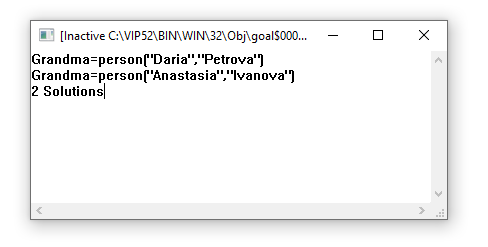
\includegraphics[scale=0.8]{img/1.png}
    \caption{grandma(person(``Arina'', ``Petrova''), Grandma).}
\end{figure}

\begin{figure}[H]
    \centering
    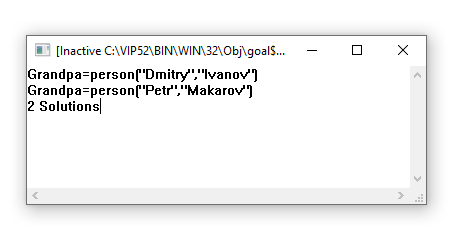
\includegraphics[scale=0.8]{img/2.png}
    \caption{grandpa(person(``Petr'', ``Ivanov''), Grandpa).}
\end{figure}

\begin{figure}[H]
    \centering
    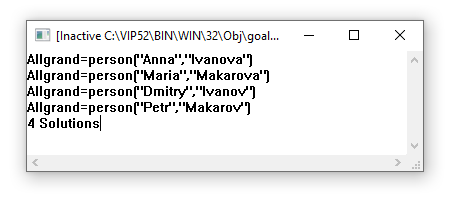
\includegraphics[scale=0.8]{img/3.png}
    \caption{allgrand(person(``Maria'', ``Petrova''), Allgrand).}
\end{figure}

\begin{figure}[H]
    \centering
    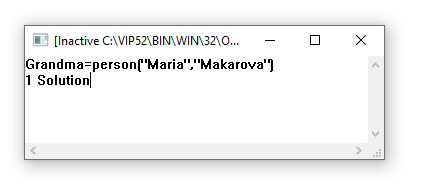
\includegraphics[scale=0.8]{img/4.png}
    \caption{grandmaMother(person(``Alex'', ``Ivanov''), Grandma).}
\end{figure}

\begin{figure}[H]
    \centering
    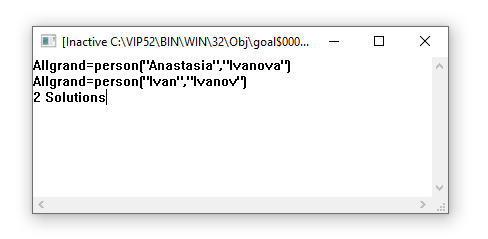
\includegraphics[scale=0.8]{img/5.png}
    \caption{allgrandMother(person(``Arina'', ``Petrova''), Allgrand).}
\end{figure}
